\section{Introduction}

The previous chapter established that code coverage, while effective, provides an incomplete view of program behavior.
This chapter presents \lool, an approach tailored specifically to compiler testing that addresses these limitations by using the compiler's own optimization log as a coverage signal.

Despite being complex software themselves, the correctness of compilers is even more important than the correctness of other software, given that bugs in the compiler can silently propagate to every program it compiles.
Yet testing compilers is challenging precisely because the interesting behaviors (optimization interactions, corner cases in code generation) are difficult to trigger with random inputs and difficult to detect with generic coverage metrics.

\lool addresses this challenge by leveraging a unique property of compilers: they already record which optimizations they perform.
By treating these optimization events as coverage features, \lool can guide input generation toward rare optimization combinations that are likely to expose bugs.

\pgfplotsset{
    optimizationchart/.style={
        width=0.9\textwidth,
        height=13cm,
        xlabel={Count},
        ylabel={},
        yticklabel style={font=\footnotesize\propernamedecl},
        y axis line style={opacity=0},
        axis x line*=bottom,
        tick align=outside,
        enlarge y limits={0.03},
        bar width=10pt,
        y=14pt,
        xminorticks=false,
        axis lines*=left,
    },
    optimizationbar/.style={
        fill=gray!20,
        draw=black,
        line width=0.4pt,
    },
}
\tikzset{
    optimizationlabel/.style={
        anchor=center,
        font=\footnotesize,
    },
}
\begin{figure}[t]
    \centering
    \resizebox{\textwidth}{!}{% Auto-generated by optimizationcounts.py
% Customize styles in importing document:
%   \pgfplotsset{optimizationbar/.style={...}}
%   \tikzset{optimizationlabel/.style={...}}
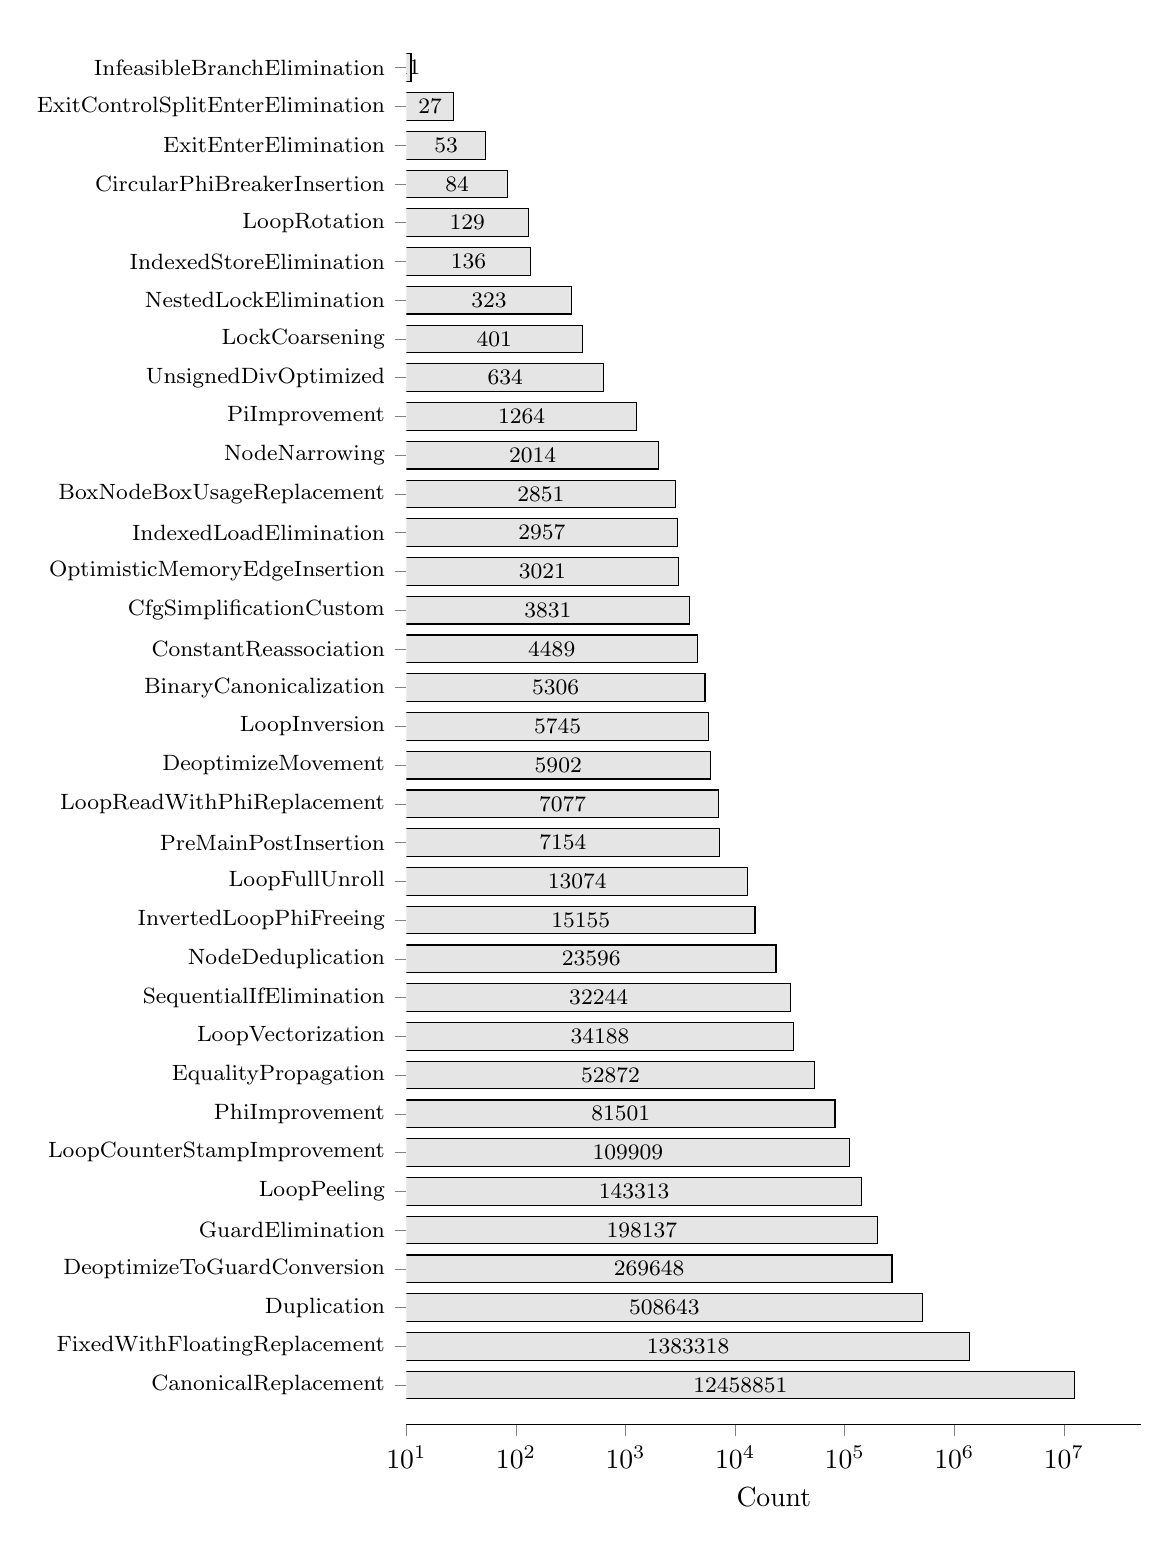
\begin{tikzpicture}
\begin{axis}[
    xbar,
    xmode=log,
    xmin=10,
    ytick=data,
    yticklabels={
        CanonicalReplacement,
        FixedWithFloatingReplacement,
        Duplication,
        DeoptimizeToGuardConversion,
        GuardElimination,
        LoopPeeling,
        LoopCounterStampImprovement,
        PhiImprovement,
        EqualityPropagation,
        LoopVectorization,
        SequentialIfElimination,
        NodeDeduplication,
        InvertedLoopPhiFreeing,
        LoopFullUnroll,
        PreMainPostInsertion,
        LoopReadWithPhiReplacement,
        DeoptimizeMovement,
        LoopInversion,
        BinaryCanonicalization,
        ConstantReassociation,
        CfgSimplificationCustom,
        OptimisticMemoryEdgeInsertion,
        IndexedLoadElimination,
        BoxNodeBoxUsageReplacement,
        NodeNarrowing,
        PiImprovement,
        UnsignedDivOptimized,
        LockCoarsening,
        NestedLockElimination,
        IndexedStoreElimination,
        LoopRotation,
        CircularPhiBreakerInsertion,
        ExitEnterElimination,
        ExitControlSplitEnterElimination,
        InfeasibleBranchElimination
    },
    optimizationchart,  % apply custom style
]
\addplot+[optimizationbar] coordinates {
    (12458851,0)
    (1383318,1)
    (508643,2)
    (269648,3)
    (198137,4)
    (143313,5)
    (109909,6)
    (81501,7)
    (52872,8)
    (34188,9)
    (32244,10)
    (23596,11)
    (15155,12)
    (13074,13)
    (7154,14)
    (7077,15)
    (5902,16)
    (5745,17)
    (5306,18)
    (4489,19)
    (3831,20)
    (3021,21)
    (2957,22)
    (2851,23)
    (2014,24)
    (1264,25)
    (634,26)
    (401,27)
    (323,28)
    (136,29)
    (129,30)
    (84,31)
    (53,32)
    (27,33)
    (11,34)
};

% Centered labels (positions pre-calculated)
\node[optimizationlabel] at (axis cs:11161.92,0) {\num{12458851}};
\node[optimizationlabel] at (axis cs:3719.30,1) {\num{1383318}};
\node[optimizationlabel] at (axis cs:2255.31,2) {\num{508643}};
\node[optimizationlabel] at (axis cs:1642.10,3) {\num{269648}};
\node[optimizationlabel] at (axis cs:1407.61,4) {\num{198137}};
\node[optimizationlabel] at (axis cs:1197.13,5) {\num{143313}};
\node[optimizationlabel] at (axis cs:1048.37,6) {\num{109909}};
\node[optimizationlabel] at (axis cs:902.78,7) {\num{81501}};
\node[optimizationlabel] at (axis cs:727.13,8) {\num{52872}};
\node[optimizationlabel] at (axis cs:584.71,9) {\num{34188}};
\node[optimizationlabel] at (axis cs:567.84,10) {\num{32244}};
\node[optimizationlabel] at (axis cs:485.76,11) {\num{23596}};
\node[optimizationlabel] at (axis cs:389.29,12) {\num{15155}};
\node[optimizationlabel] at (axis cs:361.58,13) {\num{13074}};
\node[optimizationlabel] at (axis cs:267.47,14) {\num{7154}};
\node[optimizationlabel] at (axis cs:266.03,15) {\num{7077}};
\node[optimizationlabel] at (axis cs:242.94,16) {\num{5902}};
\node[optimizationlabel] at (axis cs:239.69,17) {\num{5745}};
\node[optimizationlabel] at (axis cs:230.35,18) {\num{5306}};
\node[optimizationlabel] at (axis cs:211.87,19) {\num{4489}};
\node[optimizationlabel] at (axis cs:195.73,20) {\num{3831}};
\node[optimizationlabel] at (axis cs:173.81,21) {\num{3021}};
\node[optimizationlabel] at (axis cs:171.96,22) {\num{2957}};
\node[optimizationlabel] at (axis cs:168.85,23) {\num{2851}};
\node[optimizationlabel] at (axis cs:141.92,24) {\num{2014}};
\node[optimizationlabel] at (axis cs:112.43,25) {\num{1264}};
\node[optimizationlabel] at (axis cs:79.62,26) {\num{634}};
\node[optimizationlabel] at (axis cs:63.32,27) {\num{401}};
\node[optimizationlabel] at (axis cs:56.83,28) {\num{323}};
\node[optimizationlabel] at (axis cs:36.88,29) {\num{136}};
\node[optimizationlabel] at (axis cs:35.92,30) {\num{129}};
\node[optimizationlabel] at (axis cs:28.98,31) {\num{84}};
\node[optimizationlabel] at (axis cs:23.02,32) {\num{53}};
\node[optimizationlabel] at (axis cs:16.43,33) {\num{27}};
\node[optimizationlabel] at (axis cs:10.49,34) {\num{11}};
\end{axis}
\end{tikzpicture}}
    \caption{Counts of selected optimizations during the compilation of \num{1000} fuzzed test cases (logarithmic axis).}\label{lool:fig:optimizations}
\end{figure}

Bugs in compilers can have a significant impact on users, especially when the symptom is not a crash, but a silent miscompilation.
Determining that a suspected program bug actually is a miscompilation is a time-consuming process for software developers.
Hand-written tests for the compiler, such as unit tests for specific components, typically cover cases the compiler engineer already considers during development, but edge cases are often overlooked.

The GraalVM compiler, a compiler for Java and other languages (\cref{lool:s:graalvm}), serves as both an \gls{AOT} and \gls{JITcomp}.
As such, bugs in the GraalVM compiler potentially have a far-reaching effect and are particularly problematic.
Being written entirely in Java, the GraalVM compiler is not affected by memory safety issues plaguing compilers written in C or \cpp.
Nonetheless, the GraalVM compiler is not immune to implementation errors, occasionally leading to miscompilations or failed assertions that lead to a crash.
An effective way to compensate for the blind spot of hand-written tests is fuzzing in general and \emph{compiler fuzzing} in particular.
Compiler fuzzing aims to cover the missing test scenarios by feeding random inputs to the compiler.
We developed a compiler fuzzing framework targeting the GraalVM compiler and, in line with related work~\cite{yang2011}, found several previously unknown bugs.

The sustained effectiveness of a compiler fuzzer depends on the capabilities of the input code generator.
The generator can trigger certain compiler optimizations only with very specific combinations of language features.
A naïve input generation approach uses a fixed probability distribution of language features to include.
A problem with this approach, however, is the small probability of certain language feature combinations occurring in a test program of limited size.
If these combinations are necessary to trigger a specific optimization, the optimization remains untested with a high probability.
Optimization frequencies vary: some trigger frequently, while others trigger only rarely.
\cref{lool:fig:optimizations} shows the execution counts for certain optimizations we recorded for one fuzzing campaign with~1000 randomly generated Java programs using the code generator's default configuration.
The least frequent optimization in this data set occurs~11 times overall.
In contrast, other optimizations occur hundreds of thousands or even millions of times on the same \num{1000} test programs.
These data suggest that the GraalVM fuzzer would profit from fuzzer guidance.

In \cref{ch:fuzzer-guidance}, we discussed how feedback can transform random exploration into a more efficient, guided process.
While code coverage is a popular form of feedback, it is less common among compiler fuzzers (see \cref{lool:s:background} for an overview of JIT compiler fuzzing).
Nevertheless, some JIT compiler fuzzers do guide input mutation using code coverage~\cite{Gross2023,Wu2023}.
Code coverage would, in principle, tell us whether certain optimizations were exercised or not.
While AFL's assembly-level instrumentation is not directly applicable to the GraalVM compiler, Java bytecode instrumentation solutions exist to achieve code coverage.
For example, the coverage instrumentation of JQF~\cite{Padhye2019a}, Jazzer~\cite{jazzer}, and Kelinci~\cite{kelinci} all operate in a similar manner to AFL's coverage instrumentation.
However, code coverage has two major drawbacks:

\begin{description}
    \item[Overhead]
    Collecting code-coverage information while fuzzing the GraalVM compiler incurs non-negligible overhead.
    In our experiments with our own coverage instrumentation, we observed a fuzzer-throughput decrease of up to 70\%.
    Although our code coverage instrumentation is not optimized for speed, a non-trivial performance overhead is to be expected.
    Apart from adding additional bytecode instructions in CPU-intensive code, the instrumentation also perturbs the JIT compilation of the instrumented code.
    \item[Merging of execution contexts]
    Existing Java code coverage solutions do not contain information about the execution \emph{context} of the covered code, such as the domain knowledge that a compiler compiles separate \emph{methods}.
    As a result, conventional coverage tools merge the coverage information of, for example, an optimization pass optimizing different methods within the same input program.
    Such merged information can tell us that on a given input program the compiler optimizations~\(X\) and~\(Y\) were exercised, but not whether optimizations~\(X\) and~\(Y\) happened during the compilation of the same method.
    In other words, code coverage merges the coverage for an entire input program, even if compiler passes execute multiple times on different parts of the input (\eg methods).
\end{description}

\begin{figure}
    % Row 1: Code blocks (top-aligned)
    \begin{minipage}[t]{0.48\linewidth}
        \centering
        \begin{minted}[fontsize=\footnotesize]{java}
int sum = 0;
for (int i = 0; i < a.length; i++) {
    if (i == 0)
        log("summing array %s", a);
    sum += a[i];
}
        \end{minted}
    \end{minipage}%
    \hfill%
    \begin{minipage}[t]{0.48\linewidth}
        \centering
        \begin{minted}[fontsize=\footnotesize]{java}
int sum = 0;
if (a.length > 0) {
    log("summing array %s", a);
    sum += a[0];
    for (int i = 1; i < a.length; i++) {
        sum += a[i];
    }
}
        \end{minted}
    \end{minipage}

    \vspace{0.5\baselineskip}

    % Row 2: Subcaptions (aligned)
    \begin{minipage}[t]{0.48\linewidth}
        \subcaption{Example loop not amenable to loop vectorization due to control flow and a method call.}
        \label{lool:fig:loop_before_peeling}
    \end{minipage}%
    \hfill%
    \begin{minipage}[t]{0.48\linewidth}
        \subcaption{Example loop after loop peeling. The remaining loop is amenable to loop vectorization.}
        \label{lool:fig:loop_after_peeling}
    \end{minipage}

    \caption{Combination of compiler optimizations.}
    \label{lool:fig:context_example}
\end{figure}


Based on these observations, we extend the GraalVM compiler fuzzer to leverage a new kind of coverage:
We propose to use the GraalVM compiler's optimization log for coverage feedback.
Our fuzzer uses the precise, domain-specific information from the optimization log as context-rich coverage to guide input generation towards rare or entirely uncovered compiler optimizations.
At the core of input generation is a genetic algorithm that uses coverage feedback to choose among different generation options.
We call the combination of optimization-log-guided feedback with genetic input generation \lool.

In contrast to code coverage, \lool has lower overhead and allows for domain-specific context sensitivity.
To understand which type of context is important in compiler fuzzing, consider the example loop in \cref{lool:fig:loop_before_peeling}.
This loop contains control flow and a method call, making the common optimization of \emph{loop vectorization} inapplicable.
However, applying \emph{loop peeling} to separate the first loop iteration from the rest produces the loop in \cref{lool:fig:loop_after_peeling}, which can be vectorized.
Such information about pairs of optimizations can be interesting.
In our experience with GraalVM, many intricate compiler bugs involve such interactions between multiple compilation phases.

Our coverage based on the optimization log can record the fact that the optimizations happened in the same \emph{method} or even on the same \emph{loop}.
Thus, a context-aware coverage metric that is aware of the context of separate compilations, and that does not merge information from separate contexts, can guide the fuzzer in the direction of such interesting optimization pairs.
